\documentclass{beamer}
\usepackage{graphicx}
\usepackage{graphics}
\usepackage{hyperref}
%\usepackage[polish]{babel}
\usepackage[OT4]{polski}
\usepackage[utf8]{inputenc}

\mode<presentation>
{
  \usetheme[english]{AMU}
	\setbeamercovered{transparent = 28}
}

\title{Rozmyte k-NN}
\subtitle{Nowatorska metoda obliczania k najbliższych sąsiadów}
\author[{K. Pokrywka, D. Jurkiewicz}]{Kuba Pokrywka, Dawid Jurkiewicz}
\date{03-03-2018}
\institute[zpjn.wmi.amu.edu.pl]{Faculty of Mathematics and Computer Science\\Department of Natural Language Processing}

\begin{document}



\begin{frame}
	\titlepage
\end{frame}

\AtBeginSection[]
{
   \begin{frame}
       \frametitle{Zarys}
       \tableofcontents[currentsection]
   \end{frame}
}
\section{Standardowy klasyfikator KNN (k-nearest neighbor}

\begin{frame}{Algorytm k-nn. Predykcja dla oberwacji $x$:}
Niech $W = \{x_1,x_2, \ldots, x_n\}$  będzie zbiorem $n$ zaetykietowanych obserwacji, $c$ oznacza liczbę klas, K będzie liczbą całkowitą, $1\leq K \leq n $, $d$ będzie miarą niepodobieństwa obiektów.
\end{frame}


\begin{frame}{Algorytm k-nn. Predykcja dla oberwacji $x$:}
\begin{enumerate}
\item Posortuj rosnąco wszystkie elementy zbioru $W$ po odległości $x_i$ od $x$ względem miary $d$.
\item Wybierz $K$ elementów z najmniejsza odległością do $x_i$ ($K$- siąsiadów)
\item Jeżeli istnieje tylko jedna najbardziej reprezentowana klasa - ta klasa jest predykcją dla elementu $x$.
\item Jeżeli jest więcej niż jedna najbardziej reprezentowana klasa, wybierz klasę o najmniejszej sumie odległości do $K$-sąsiadów,
\item Znajdź k najbliższych obserwacji ze zbioru $W$. 
\end{enumerate}
\end{frame}

\begin{frame}{Przykład}
\begin{figure}[H]
\begin{center}
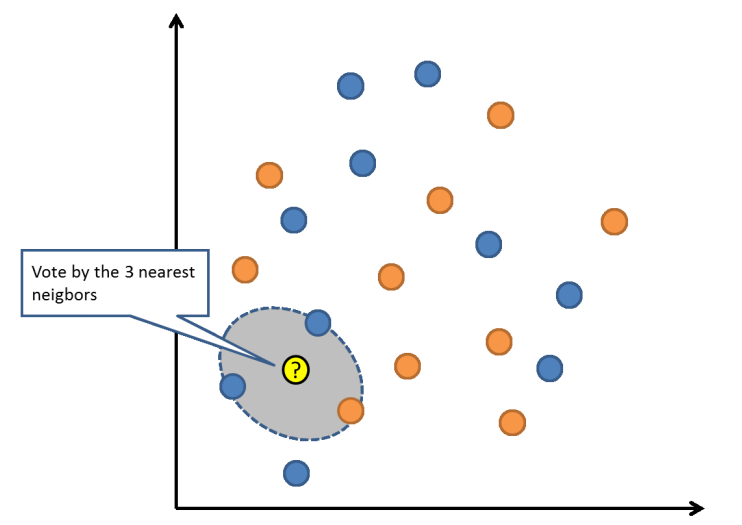
\includegraphics[scale=0.3]{knn.png}
\end{center}
\end{figure}
\end{frame}

\begin{frame}{Właściwości klasyfikatora knn}
\begin{itemize}
   \item Działa zarówno na zmiennych ilościowych jak i zmiennych jakościowych
   \item Wymaga wybrania miary niepodobieństwa
   \item Jest bardzo wrażliwy na skalowanie i normalizację cech
   \item Działa wolno, jeżeli rozmiar danych trenujących jest duży
\end{itemize}
\end{frame}

\begin{frame}{Miara niepodobieństwa obiektów}
   Funkcję $d:X\times X \rightarrow R $ nazywamy miarą niepodobieństwa, jesli
   \begin{enumerate}
       \item $d(x,y) \geq 0$ 
       \item $d(x,y) = 0$  wtedy i tylko wtedy, gdy $x = y$
       \item $d(x,y) = d(y,x)$
   \end{enumerate}
   Miara taka jest semi-metryką (nie musi spełniać warunku trójkąta)
\end{frame}

\begin{frame}{Różne miary niepodobieństwa}
\begin{itemize}
    \item metryka euklidesowa $d(x,y) = (\sum\limits_{i=1}^{p} (x_i - y_i)^2)^{\frac{1}{2}}$
    \item ważona metryka euklidesowa $d(x,y) = (\sum\limits_{i=1}^{p} \frac{1}{w_i^2}(x_i - y_i)^2)^{\frac{1}{2}}$
    \item metryka euklidesowa $d(x,y) = \sum\limits_{i=1}^{p} \left| x_i - y_i\right|$
    \item współczynnik Sneatha $d(x,y) = \frac{1}{p} \sum\limits_{i=1}^{p} I \left( x_i - y_i\right)$ (zmienne jakościowe)
\end{itemize}
\end{frame}


\begin{frame}{Normalizacja danych}
\begin{figure}[!tbp]
  \centering
  \begin{minipage}[b]{0.45\textwidth}
    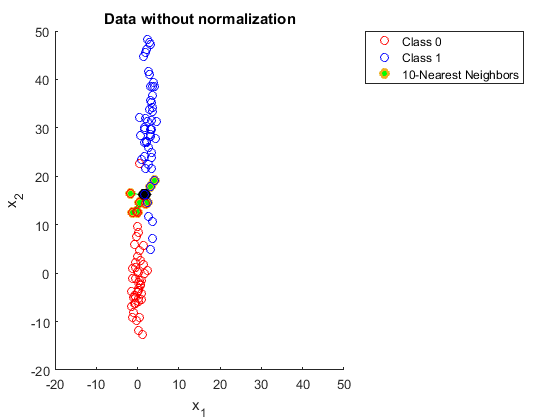
\includegraphics[width=\textwidth]{knn-ns.png}
  \end{minipage}
  \hfill
  \begin{minipage}[b]{0.45\textwidth}
    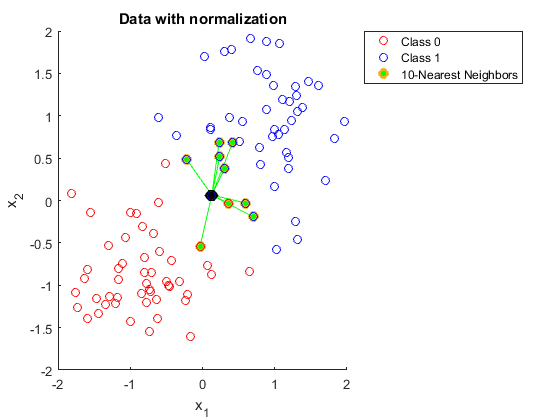
\includegraphics[width=\textwidth]{knn-s.png}
  \end{minipage}
\end{figure}
\end{frame}


\section{Macierz przynależności klas}

\begin{frame}
\frametitle{Macierz przynależności klas}
Załóżmy, że mamy zbiór obserwacji $\{x_1, \ldots, x_n\}$. Macierz przynależności obserwacji do klas $c$ oznaczmy jako $U_{c \times n}$.
Definiujemy ją jako: 
\begin{equation}
    u_{ik} = u_i(x_k)
\end{equation}    
 dla $i=1, \ldots, c$ i $k=1,\ldots,n$
 i mówimy, że $u_{ik}$ to stopień przynależności $x_k$ do klasy $i$.
\end{frame}

\section{Pseudokod}
\begin{frame}
\frametitle{Pseudokod}
	\begin{enumerate}
        \item Posortuj wszystkie elementy zbioru $W$ po odległości $x_i$ od $x$ względem miary $d$.
        \item Wybierz $K$ elementów z najmniejszą odległością do $x_i$ ($K$- siąsiadów)
        \item Policz $u_i(x)$ dla $i=1, \ldots, c$, gdzie 
	\end{enumerate}
	\vspace{2mm}
    \begin{equation}
         u_i(x) = \frac{\sum_{j=1}^{K} u_{ij} \times (\frac{1}{||x-x_j||^{2/(m-1)}})}
         {\sum_{j=1}^{K} \frac{1}{||x-x_j||^{2/(m-1)}}}   
    \end{equation}
\end{frame}	


\begin{frame}
	\frametitle{Inicjalizacja macierzy przynależności}
	\begin{enumerate}
    	\item Binarna inicjalizacja
	    \item Rozmyta inicjalizacja
	\begin{equation}
        u_j(x) = \left\{
          \begin{array}{lr}
            0.51 + 0.49 \cdot \frac{n_j}{K} & : j = i\\
            0.49 \cdot \frac{n_j}{K} & : j \neq i
          \end{array}
        \right.
	\end{equation}
	\end{enumerate}
\end{frame}	

\section{Wyniki}
\begin{frame}{Wyniki}
\begin{figure}[H]
\begin{center}
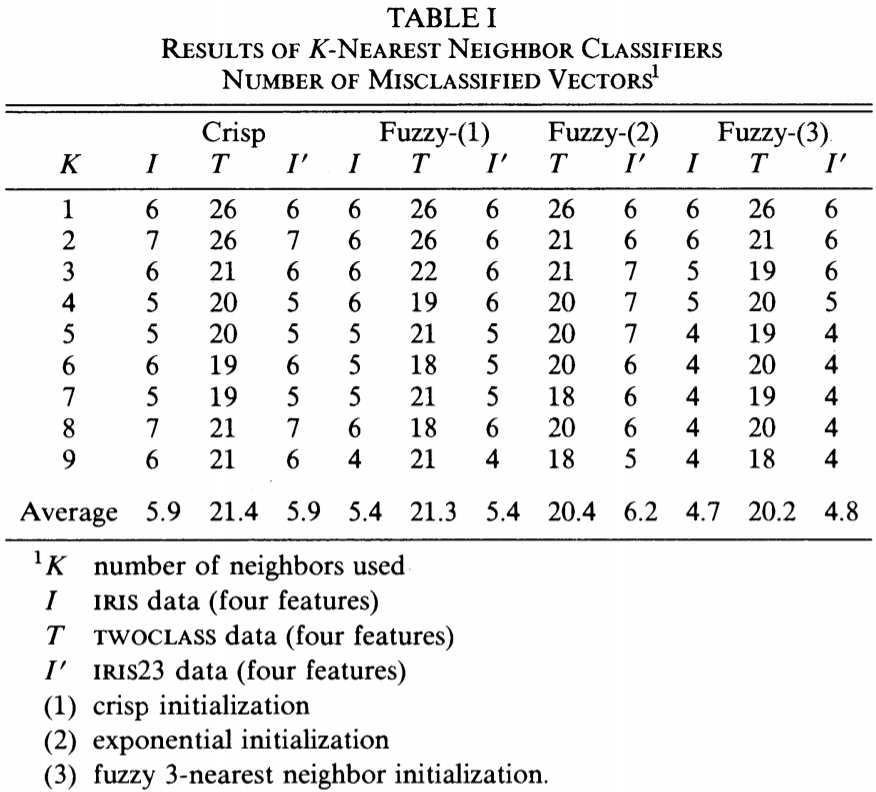
\includegraphics[scale=0.37]{wyniki_1.png}
\end{center}
\end{figure}
   
\end{frame}
\begin{frame}{Wyniki c.d.}
 \begin{figure}[!tbp]
  \centering
  \begin{minipage}[b]{0.49\textwidth}
    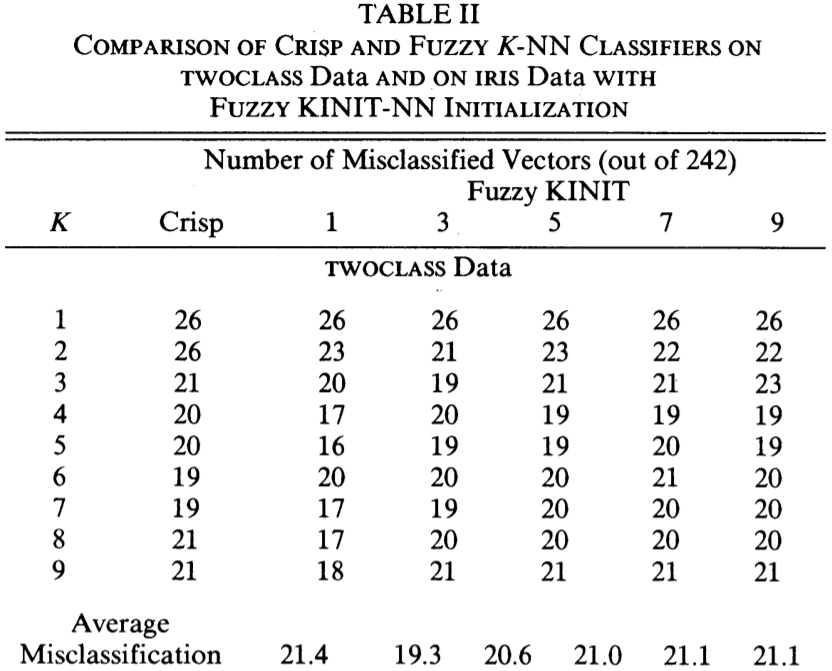
\includegraphics[width=\textwidth]{wyniki_2.png}
  \end{minipage}
  \hfill
  \begin{minipage}[b]{0.49\textwidth}
    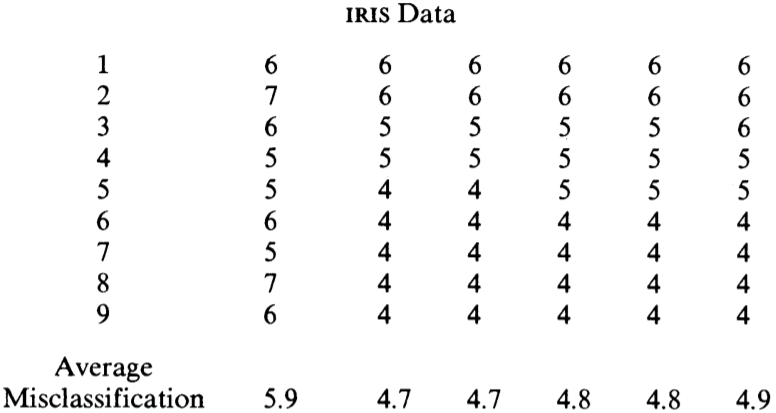
\includegraphics[width=\textwidth]{wyniki_3.png}
  \end{minipage}
\end{figure}
\end{frame}



\begin{frame}

\begin{thebibliography}{9}

\bibitem{gorecki}
Tomasz Górecki, Statystyczne Systemu Uczące, http://drizzt.home.amu.edu.pl/images/DSSU/W8.pdf
\end{thebibliography}

\end{frame}



\end{document}
